
\begin{frame}{Introdução}
    \begin{columns}[T]
        \begin{column}{.5\textwidth}
            \begin{itemize}
                \item Cloud Computing
            \end{itemize}
        \end{column}

        \begin{column}{.5\textwidth}
            \begin{figure}
                \centering
                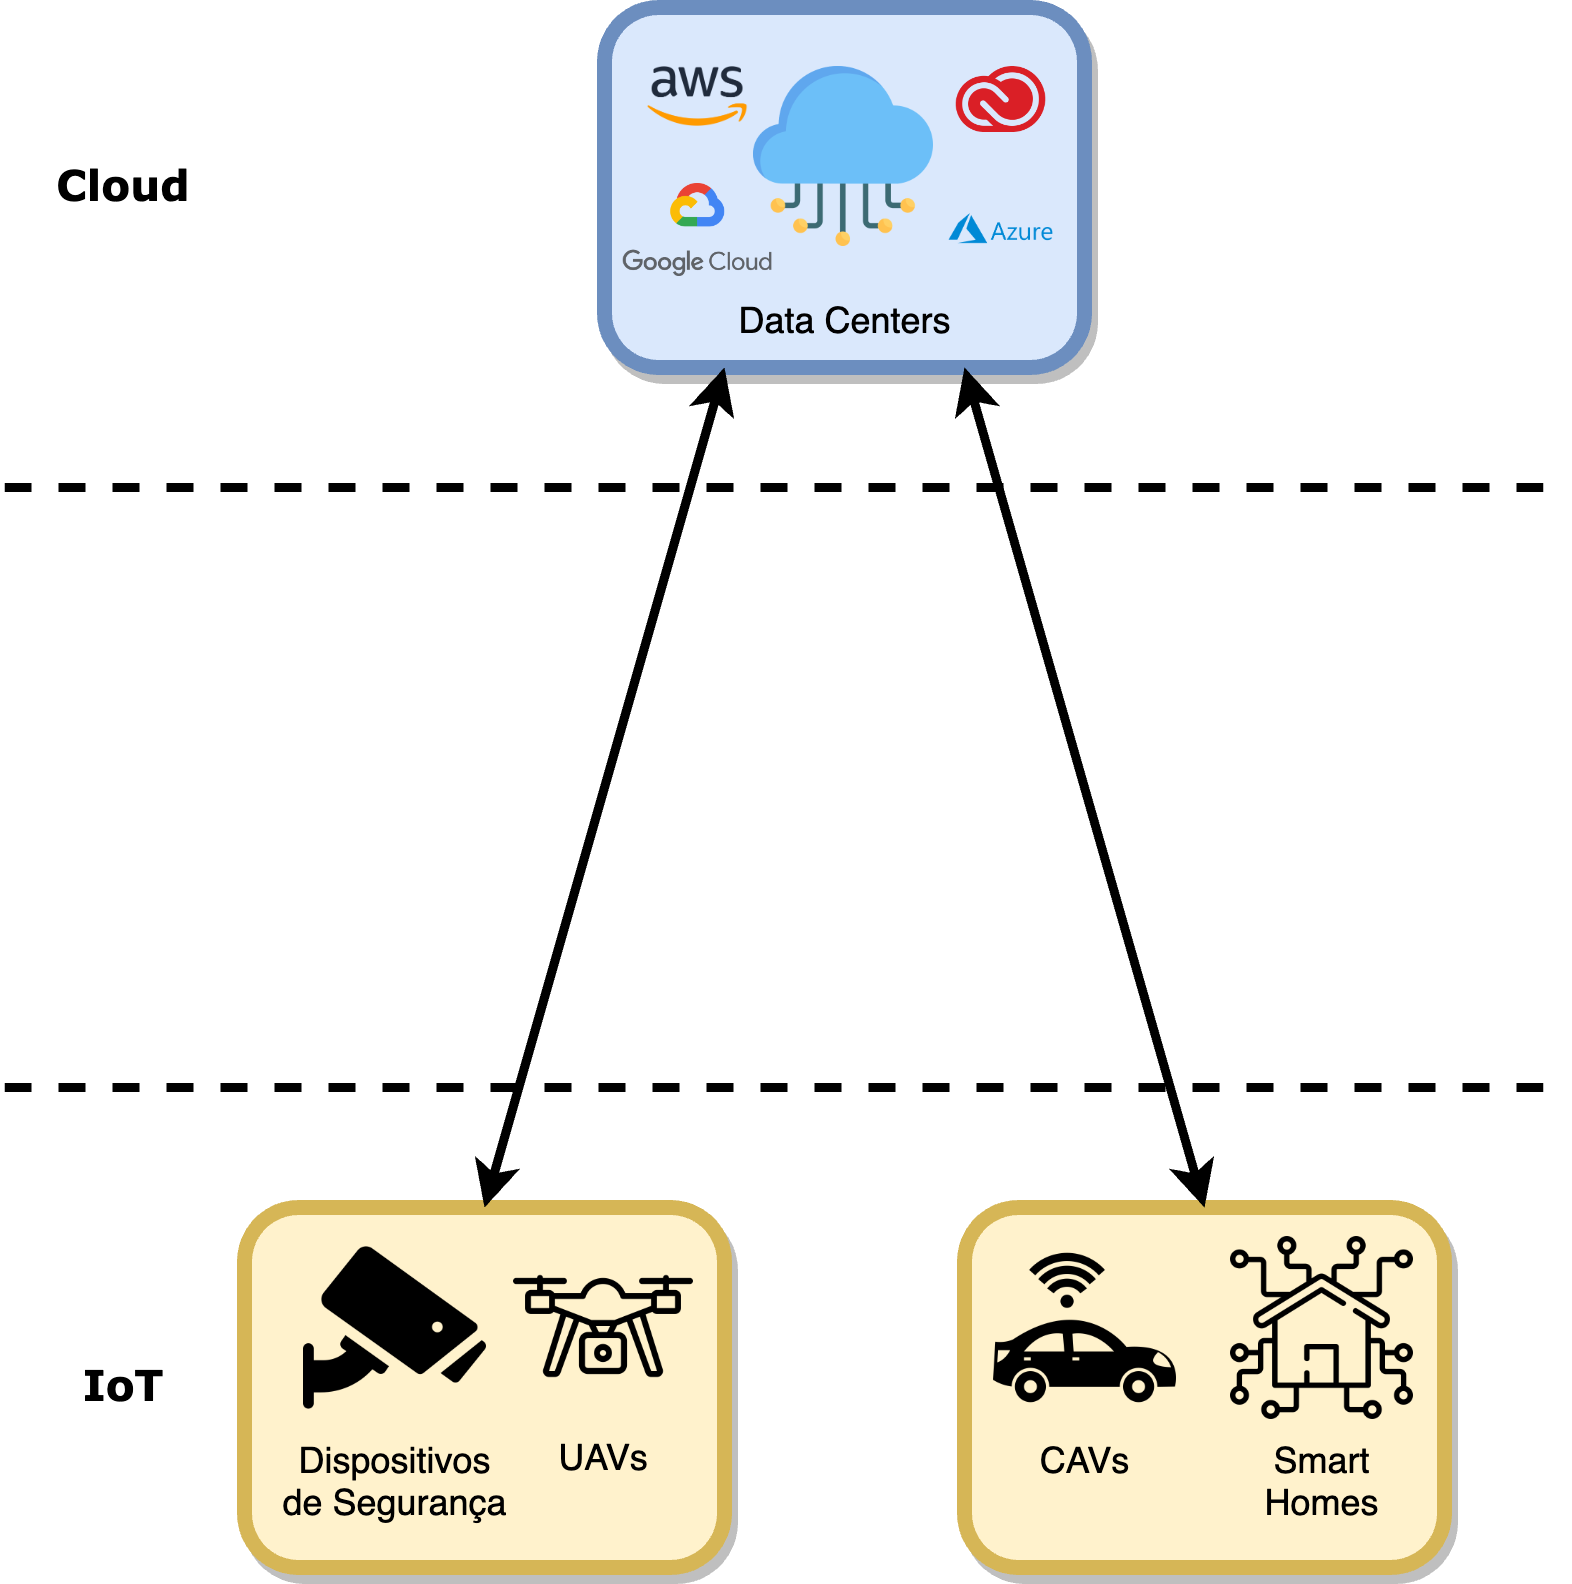
\includegraphics[width=\textwidth]{Figuras/TCC Cloud IoT.png}
            \end{figure}
        \end{column}
    \end{columns}
\end{frame}

\begin{frame}{Introdução}
    \begin{columns}[T]
        \begin{column}{.5\textwidth}
            \begin{itemize}
                \item Cloud Computing
                \item Edge-Cloud Continuum
                \begin{itemize}
                    \item[--] Escalonamento de recursos
                \end{itemize}
            \end{itemize}
        \end{column}

        \begin{column}{.5\textwidth}
            \begin{figure}
                \centering
                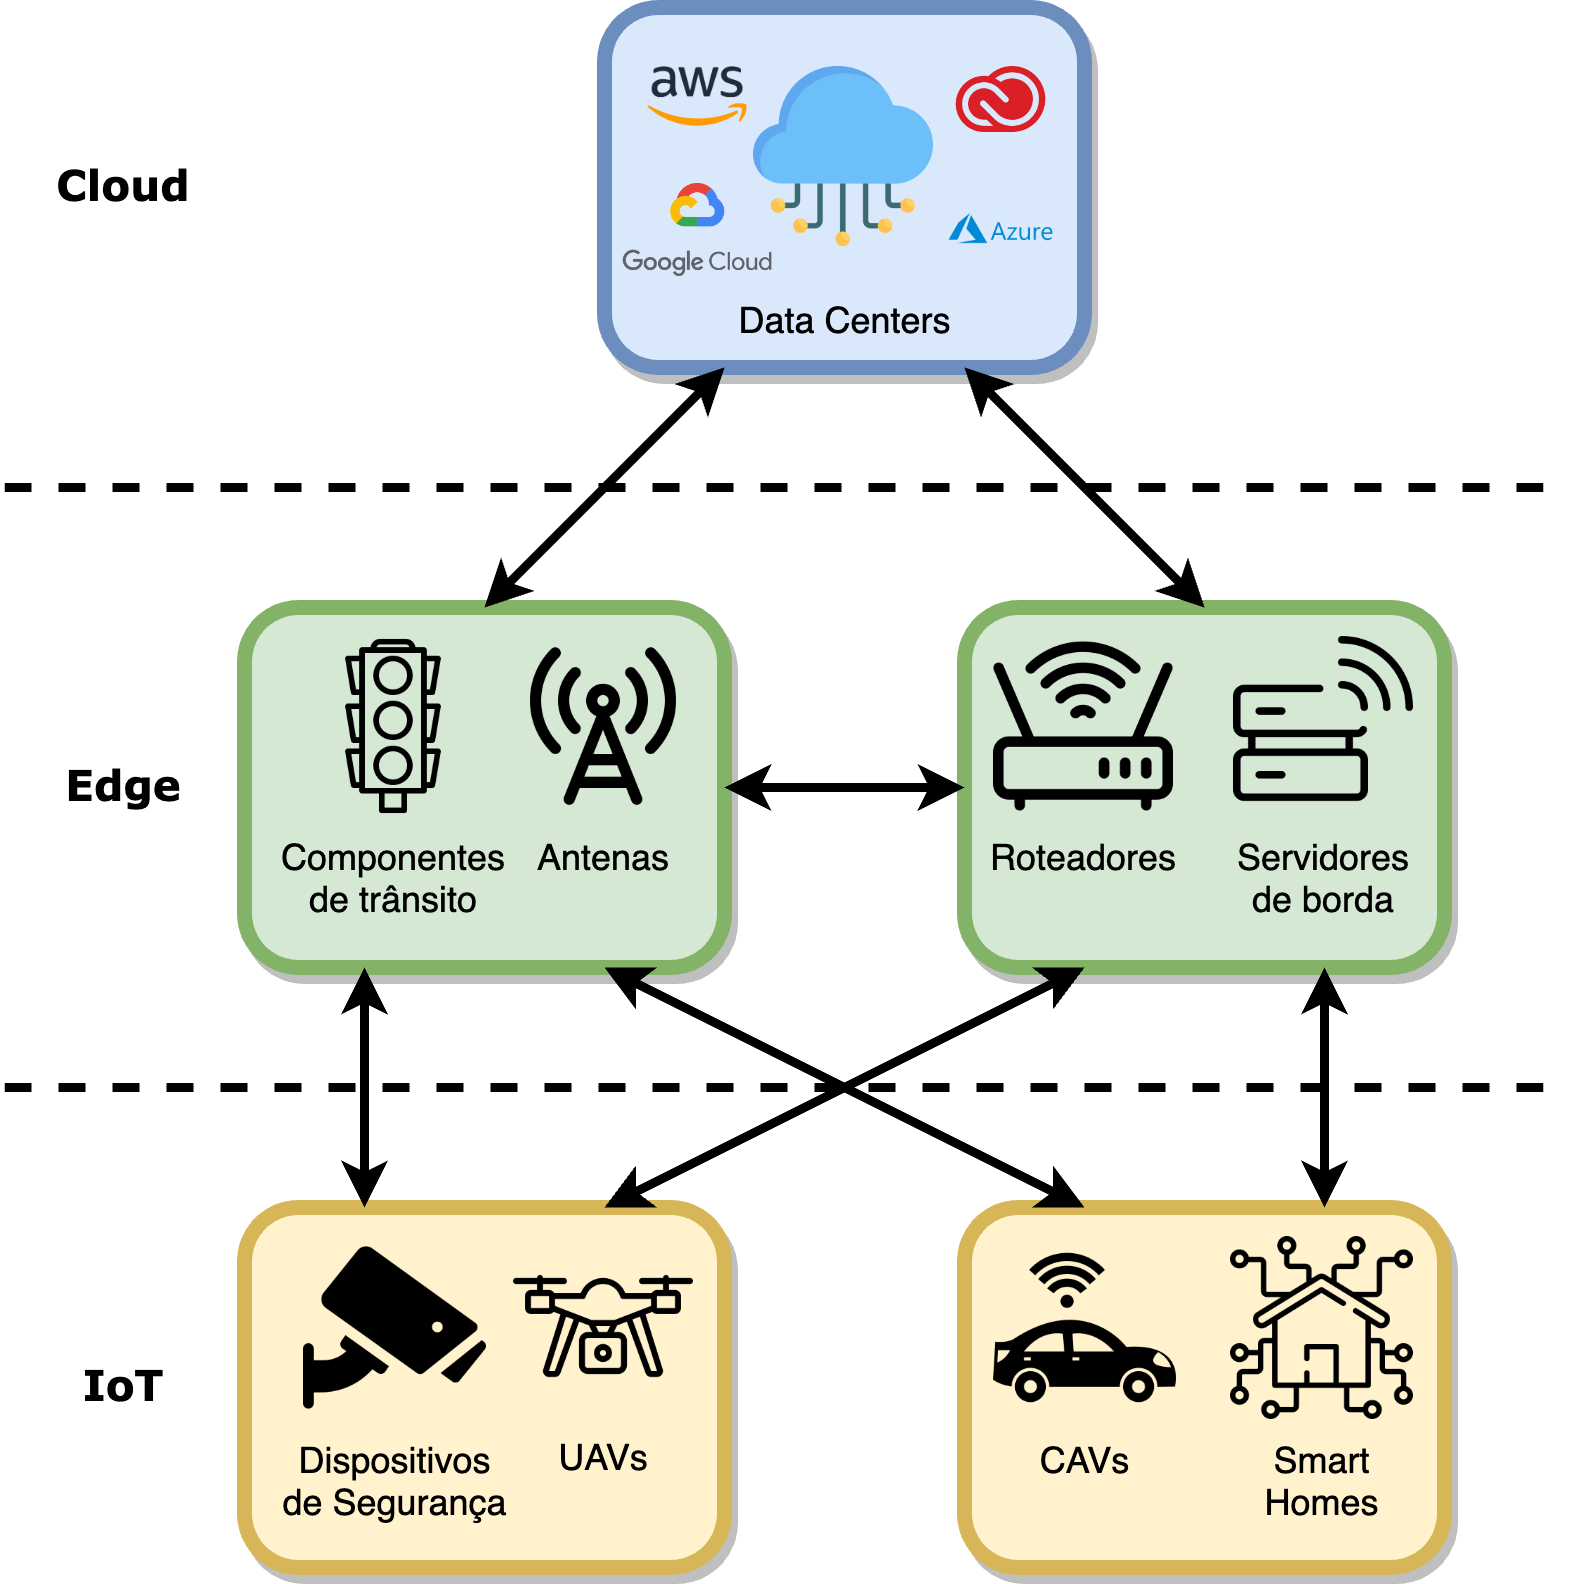
\includegraphics[width=\textwidth]{Figuras/TCC Edge Cloud IoT.png}
            \end{figure}
        \end{column}
    \end{columns}
\end{frame}
